\documentclass[a4paper, 11pt, twoside]{article}

\usepackage[brazilian]{babel}
\usepackage[utf8]{inputenc}
\usepackage[T1]{fontenc}
\usepackage{fixltx2e}
\usepackage{amsmath}
\usepackage{amssymb}
\usepackage{graphicx}
\usepackage{float}
\usepackage{a4wide}
\usepackage{multicol}
\usepackage{xcolor}
\usepackage{makeidx}
\usepackage{hyperref}
\usepackage{textcomp}

\newcommand{\HRule}{\rule{\linewidth}{0.5mm}}

\begin{document}

\hypersetup{backref,pdfpagemode=FullScreen,colorlinks=true}

\begin{titlepage}

\begin{center}
% Upper part of the page

%\includegraphics[width=0.15\textwidth]{./usp.jpg}\\[1 cm]

\textsc{\LARGE Universidade de São Paulo}\\
\textsc{\Large Pró-Reitoria de Graduação}\\
\textsc{\Large Curso de Ciências Moleculares}\\[1.5cm]
\textsc{\Large Relatório Final de Iniciação Científica}\\[0.5cm]

% Title
\HRule \\[0.4cm]
{ \LARGE \bfseries Interfaces entre o Usuário e Sistemas Musicais Multiagentes}\\[0.4cm]

\HRule \\[1.5cm]

% Author and supervisor
\begin{minipage}{0.4\textwidth}
\begin{flushleft} \normalsize
\emph{Autor:}\\
Pedro H. R. \textsc{Bruel} \\
\vspace{0.3cm}
\emph{Email:}\\
pedro.bruel@gmail.com \\
\vspace{0.3cm}
\emph{Telefone: 97587-2511}\\
\vspace{0.3cm}
\emph{Turma: 20}\\
\end{flushleft}
\end{minipage}
\begin{minipage}{0.5\textwidth}
\begin{flushright} \normalsize
\emph{Orientador:} \\
Prof Dr Marcelo \textsc{Queiroz} \\
\vspace{0.3cm}
\emph{Email:}\\
mqz@ime.usp.br \\
\vspace{0.3cm}
\emph{Unidade: }\\
Instituto de Matemática e Estatística \\
\vspace{0.3cm}
\emph{Departamento: }\\
Ciência da Computação\\
\end{flushright}
\end{minipage}
\vfill
% Bottom of the page
{\large 2º Semestre de 2013}

\end{center}

\end{titlepage}


\tableofcontents
\newpage

\begin{abstract}
\line(1,0){350}

A adaptabilidade em tempo real e o potencial de modelagem de sistemas complexos
são características de Sistemas Multiagentes, que têm variadas aplicações no 
contexto musical. A ferramenta de criação musical e linguagem de programação 
Pure Data (Pd) é tradicionalmente utilizada por músicos em performances 
musicais. Este projeto produziu uma integração do arcabouço para Sistemas
Multiagentes Musicais Ensemble - implementado pelo Grupo de Computação Musical 
do IME/USP - com a libpd, uma infraestrutura do tipo API para Pure Data. 
A integração procura facilitar a utilização do arcabouço por usuários 
não programadores. A interface é uma extensão do Arcabouço Ensemble,
e permite desenvolver aplicações do Arcabouço através do ambiente gráfico
do Pure Data.

\line(1,0){350}
\end{abstract}

\begin{multicols}{2}

\section{Introdução}

Este relatório descreve e detalha as atividades desenvolvidas no período de 
Fevereiro a Julho de 2014, sumarizadas a seguir.

O aluno apresentou um seminário sobre o trabalho desenvolvido na elaboração da 
interface entre a linguagem de programação Pure Data e o Arcabouço Ensemble, 
no ciclo aberto de seminários do Grupo de Computação Musical.

Elaborou-se um protocolo de comunicação entre o Arcabouço Ensemble e o
Pure Data, permitindo a comunicação entre \textit{patches} e o Arcabouço.

A interface de comunicação básica implementada no semestre passado foi
largamente extendida durante este semestre, permitindo a definição de
Agentes Musicais, seus Raciocínios e Componentes e até aplicações
completas do Arcabouço Ensemble através de \textit{patches} Pure Data.

Submetemos um artigo para a Conferência Conjunta ICMC/SMC 2014~\cite{},
detalhando o protocolo e a interface desenvolvidos. O artigo foi aceito
para publicação e apresentação oral na Conferência.

As próximas seções apresentam o detalhamento destas atividades.

\section{O Protocolo}

\section{A Interface}

\subsection{Classes Java}

Esta seção apresenta uma descrição detalhada da interface Ensemble-Pd,
justificando as principais classes Java utilizadas, expondo suas 
interrelações e contextualizando seu papel no funcionamento de aplicações
do Ensemble.

\subsubsection{PdAgent}

Esta classe é uma extensão da classe \textbf{MusicalAgent} do Ensemble,
e suas instâncias representam agentes musicais numa aplicação.
O mapeamento de um agente definido num \textit{patch} e sua representação no 
Ensemble é feito através dessa classe.

Os componentes de um Agente, como Raciocínio, Atuadores e Sensores, são
adicionados a \textbf{PdAgent} através de mensagens definidas dentro do
\textit{patch}. Atuadores e Sensores são representados pelas classes 
\textbf{PdActuator} e \textbf{PdSensor}, respectivamente.

O Servidor de Eventos de uma aplicação Ensemble-Pd é responsável por garantir 
que a representação de um Agente num \textit{patch} receba e envie Eventos, 
Mensagens e Áudio de e para o Ambiente Virtual e outros Agentes. Isso é feito
através de Sensores e Atuadores especiais, inseridos por padrão em instâncias
de \textbf{PdAgent}, e que permitem essa comunicação.

\subsubsection{PdReasoning}

O raciocínio de um Agente numa aplicação Ensemble-Pd é definido dentro do
\textit{subpatch}/abstração correspondente a esse Agente, e consiste de
uma aplicação Pd que pode conter qualquer objeto Pd utilizado em aplicações
tradicionais. De dentro do \textit{patch} de Raciocínio, o programador Pd tem 
acesso à informação recebida pelo Agente através dos Sensores que ele definiu,
podendo utilizar os recursos de Processamento de Sinais implementados no Pure
Data para produzir e processar amostras de áudio e demais informações 
recebidas, e pode atuar no Ambiente Virtual através dos Atuadores do Agente.

\subsubsection{PdEvent}

Esta classe encapsula, no funcionamento de uma aplicação Ensemble,
as mensagens e informações provenientes e destinadas a \textit{patches} Pd.

Os tipos manipulados por esta classe são \textbf{PdFloat}, \textbf{PdMessage} e
\textbf{PdAudioBlock}, que por sua vez encapsulam os diferentes tipos de dados
tratados pelo Pure Data.

\subsubsection{PdServer}

Esta é a principal classe do ponto de vista da sincronização 
e mapeamento entre \textit{patches} e aplicações Ensemble.
Ela é quem centraliza e coordena a execução de um \textit{patch}, utilizando
a classe \textbf{PdProcessor}, e processa as mensagens e dados recebidos do Pd 
através da classe \textbf{PdReceiver}, produzindo Eventos para os Sensores 
dos Agentes a que essas mensagens se destinam.

Além disso, é ela quem processa os Eventos enviados por Atuadores de Agentes,
reproduzindo no \textit{patch} as mudanças feitas pelos Agentes.

\subsubsection{PdReceiver}

Esta é uma extensão da classe \textbf{PdDispatcher} contida na implementação
Java da libpd, e encapsula as funções de \textit{callback} usadas na
comunicação entre \textit{patches} e aplicações que usam a libpd.

Esta classe também é responsável por registrar e gerenciar símbolos
usados na comunicação do Ensemble com o \textit{patch}, centralizando
o envio e recebimento de mensagens, áudio e demais informações.

\subsubsection{PdAudioBlock}

Durante a implementação da interface, desenvolvemos duas diferentes estratégias
para a transferência de amostras de áudio entre o \textit{patch} e o Ensemble, 
uma centralizada e uma distribuída, finalmente optando pela centralização 
do ciclo de processamento na classe \textbf{PdServer}.

A estratégia distribuída consistia na descentralização dos ciclos de
processamento da libpd, permitindo que cada Raciocínio de um Agente
inserido numa aplicação processasse seu \textit{subpatch} independentemente,
tratando suas próprias mensagens e amostras de áudio separadamente.

Essa estratégia gera problemas de sincronização de Eventos e Áudio,
decorrentes do funcionamento dos dois softwares envolvidos.

As amostras de áudio produzidas num mesmo momento pelos Agentes 
num \textit{patch} devem ser tocadas como seriam num \textit{patch}
processado pelo Pd, e as mensagens enviadas pelos Agentes devem obedecer
uma sequência definida pelo Raciocínio, também definido num \textit{patch}.
Se cada Agente é capaz de processar o \textit{patch} de aplicação
no seu ciclo de processamento no Ensemble, não é possível garantir que ele
não receberá ou enviará Eventos ou Áudio somente após todos os outros Agentes 
recebam seu "turno" de Eventos, pois o controle de tempo execução dos Agentes 
é feito pelo middleware JADE, e não tem conexão com o ciclo de processamento
da libpd.

Como o \textit{patch} de configuração de aplicação é único, o controle de
processamento descentralizado produz desencontros nas amostras de Áudio, 
e também no fluxo de Eventos da aplicação.

A solução de processamento centralizado resolve estes problemas utilizando
as abstrações Pd \textbf{act\textasciitilde} e \textbf{sense\textasciitilde},
e as classes Java \textbf{PdAudioBlock} e \textbf{PdAudioBlockStream}.

Essas classes representam um bloco de processamento do Pure Data, e um
encadeamento temporal desses blocos, respectivamente. Elas permitem
receber amostras de Áudio de cada Atuador independentemente, e enviar
amostras a Sensores de forma sincronizada, pois cada Sensor e Atuador
tem seu próprio \textbf{PdAudioBlockStream}.

O Servidor de Eventos pode então enviar e receber Áudio e Eventos de Agentes,
mantendo a sincronia entre a execução do Ensemble e o processamento 
do \textit{patch}.

\subsection{Abstrações no Pure Data}

\subsubsection{act\textasciitilde e sense\textasciitilde}

\subsubsection{read\_memory\textasciitilde e read\_fact}

\section{Pure Data}

A linguagem de programação visual Pure Data, ou \textbf{Pd}~\cite{puckette97}, 
é uma ferramenta tradicionalmente utilizada por músicos no processo de criação
e composição de material musical~\cite{leandro11}. 

A entrada de um programa em Pure Data é tratada como
um fluxo de informação, que é direcionado e processado
em blocos, produzindo uma saída em tempo real.

A linguagem fornece abstrações de alto nível que encapsulam
diversas funcionalidades, como operações matemáticas,
de entrada/saída, e outras operações sobre sinais.

Um programa é composto pela conexão dessas
funcionalidades, ou objetos, e é chamado de patch.

\begin{table}[H]
    \centering
    \begin{tabular}{|l|}\hline
        Pure Data\\[0.07in]
        \begin{tabular}{|l|}\hline
            Interface Gráfica\\\hline
            \\
            Múltiplos Patches;\\
            Threading;\\
            Controle Temporal;\\
            Processamento de Sinais;\\
            \\
            \hline
            API de Áudio\\[0.07in]
            \hline
        \end{tabular}
        \\
        \\
        \hline
    \end{tabular}    
    \caption{Estrutura do Pure Data - Execução Independente.}
\end{table}

Trabalhando com entradas (\textit{inlets}) e saídas (\textit{outlets}) ligadas 
entre si através de \textit{patches}, é possível estruturar blocos de 
processamento e gerenciar fluxos de áudio ao longo do tempo.

O Pure Data fornece um ambiente de desenvolvimento
capaz de execução independente, e ferramentas potentes
voltadas a aplicações sonoras e musicais, porém essas 
características estão amarradas a interfaces de usuário 
e APIs de áudio que são direcionadas a certos formatos de aplicação.

A Tabela 1 ilustra a estrutura de uma instância do Pure Data
enquanto executa e edita \textit{patches}. Além da interface
gráfica e da saída de áudio, é possível trocar informação com um patch através
de mensagens OSC, entrada/saída de amostras e mensagens de outro \textit{patch}.

\subsection{libpd}

A libpd é uma biblioteca de funções que permite utilizar patches e 
funcionalidades do Pure Data no contexto de outras aplicações,
encapsulando e simplificando a interface do Pure Data com o
desenvolvedor e com outras linguagens de programação~\cite{libpd1}.

Uma aplicação que utiliza a libpd deve se preocupar com a inicialização do Pd
e de suas funções para callback, e com a chamada dos métodos 
de processamento nos momentos em que precisar de amostras de áudio.

Ao encapsular a interface do Pure Data, a libpd
permite a utilização de funções nativas, patches e funções de 
bibliotecas externas do Pure Data no contexto de aplicações em 
diferentes linguagens e plataformas.

Nesse processo, são removidas algumas das características
que dão independência à execução do Pd, e torna-se 
mais fácil utilizar \textit{patches} no contexto de outras aplicações.

Um \textit{patch} pode ser utilizado como um gerador de áudio,
que modifica sua saída de acordo com entradas fornecidas pela
aplicação que executa o \textit{patch}, produzindo amostras 
dependentes do contexto dessa aplicação, e que serão utilizadas 
por ela quando necessário.

Outro exemplo de utilização de \textit{patches} é o processamento de
amostras de áudio produzidas pela aplicação, e neste caso é possível
pensar no \textit{patch} como uma biblioteca de Processamento Digital
de Sinais, que pode receber amostras de áudio e sinais de controle e produzir
amostras processadas, que serão utilizadas pela aplicação.

% Sobre "interface com o usuário", o que quis dizer foi isso:
Um \textit{patch} pode ainda ser utilizado de forma estática, como 
mecanismo de controle e configuração da aplicação, enviando mensagens
sem necessariamente processar ou produzir áudio.

A Tabela 2 ilustra o encapsulamento do Pure Data através dos
métodos e abstrações implementados pela libpd. O código cliente
mantém controle sobre sua execução, e comanda os ciclos de 
processamento do Pd, definindo a taxa de amostragem, tamanho
de bloco, e quantos blocos serão recebidos por ciclo de processamento.

\begin{table}[H]
    \centering
    \begin{tabular}{|l|}\hline
        Código Cliente\\[0.07in]
        \begin{tabular}{|l|}\hline
            GUI do Código Cliente\\\hline
            \\
            Código de Alto Nível;\\
            Threading;\\
            Controle Temporal;\\
            \\
            \begin{tabular}{|l|}\hline
                libpd\\[0.07in]
                \begin{tabular}{|l|}\hline
                    Pure Data\\\hline
                    \\
                    Múltiplos Patches;\\
                    Processamento de Sinais;\\
                    \\
                    \hline
                \end{tabular}
                \\
                \\
                \hline
            \end{tabular}
            \\
            \\
            \hline
            API de Áudio do Código Cliente\\[0.07in]
            \hline
        \end{tabular}
        \\
        \\
        \hline
    \end{tabular}
        \caption{Estrutura de Código Cliente encapsulo o Pd com a libp.}
\end{table}

O código cliente pode então tratar um patch como
uma "caixa-preta" que recebe e devolve amostras
e dados, desde que o patch respeite convenções
de símbolos \textit{send} e \textit{receive}.

Durante o semestre, o aluno desenvolveu um repositório git~\cite{ensemble_git}
com exemplos de uso da libpd junto às linguagens C e Java,
adquirindo familiaridade e prática com o uso desta biblioteca.

% Retirei a seção de aplicações da libpd. Ela estava aqui porque eu tinha
% pesquisado sobre essas aplicações para o seminário, e achei que elas
% ajudavam a contextualizar a libpd, mas vi que já apresentei bastantes usos
% do Pd no relatório passado.

\section{Ensemble}

O Ensemble é um arcabouço para a construção de Sistemas Musicais Multiagentes, 
desenvolvido e descrito por Thomaz~\cite{leandro11} e 
Santiago~\cite{santiago12}, e tem como público alvo a comunidade de músicos que
utiliza o computador como ferramenta de criação musical, fornecendo os serviços
e ferramentas necessários para a criação de Sistemas Musicais Multiagentes. 

O arcabouço contém uma série de classes que permitem fácil extensão pelo
código cliente, além de um complexo sistema interno para
controle temporal e de execução.

A programação de novos componentes para o Ensemble requer conhecimento de seu 
funcionamento, e deve seguir as convenções de programação do arcabouço. 

\subsection{Arquitetura}

A arquitetura~\cite{leandro11} do Ensemble segue o paradigma de programação 
orientada a objetos, exigindo uma linguagem capaz de implementá-lo.

A presente implementação do Ensemble foi codificada em linguagem Java, a fim de
permitir que aplicações musicais possam ser executadas em plataformas distintas

A arquitetura utiliza o middleware para sistemas multiagentes JADE~\cite{belli99}, 
que provê a infraestrutura necessária para manter o ciclo de vida dos Agentes e
controlar a troca de mensagens entre eles.

São utilizadas principalmente três funcionalidades do JADE na implementação do
Ensemble, o serviço de agendamento de tarefas, o mecanismo de troca de mensagem
entre os agentes e o serviço de diretório.

\subsubsection{Arquitetura de Aplicação}

Uma aplicação do Ensemble deve estender e utilizar um conjunto de classes
específicas, dependente das funcionalidades desejadas. Apesar disso,
toda aplicação deve ser composta de alguns componentes-chave. 

É necessário definir um Agente Ambiente e um Mundo, que serão as classes
utilizadas pelo Ensemble para controlar a execução da aplicação,
e fornecerão um ambiente virtual específico para os Agentes Musicais.

A aplicação pode então adicionar Agentes Musicais e seus componentes, 
como Raciocínios, Bases de Conhecimento, Atuadores e Sensores, e esses
componentes também terão sua execução controlada pelo Ensemble, pois
estarão vinculados a um Agente Ambiente.

\begin{figure}[H]
  \centering
  %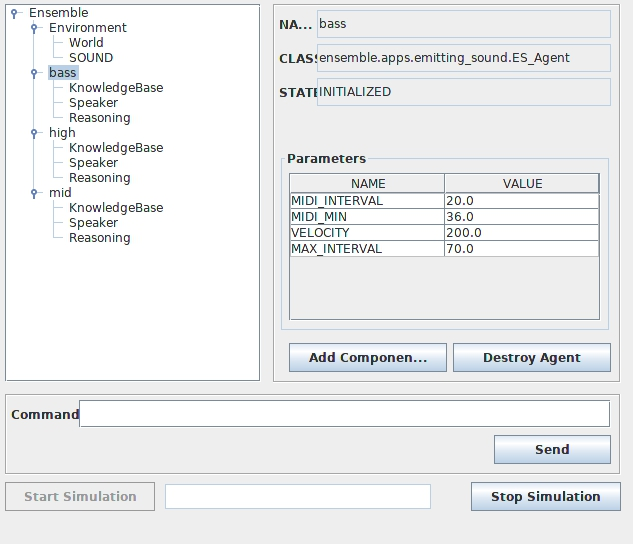
\includegraphics[scale=0.35]{./ensemble_sniffer_ext.jpg}
  \caption{Exemplo de Extensão do Ensemble}
  \label{fig2}
\end{figure}

A Figura 1 demonstra, através do Sniffer, a arquitetura de uma extensão simples
do arcabouço, que conta com três Agentes emissores de notas
MIDI no Ambiente Virtual. Note a Base de Conhecimentos, 
o Raciocínio e um Atuador cadastrados
para cada Agente Musical. Ainda é possível observar os
parâmetros contidos na Base de Conhecimentos de cada
Agente, referentes às características do som que eles emitem.

O usuário deve escolher a interface de áudio que vai utilizar,
e definir os tipos de eventos que serão tratados por sua aplicação.
Isso é feito através da extensão das classes de Servidores de Eventos.
As classes de Atuadores e Sensores definirão o tratamento dos tipos
de eventos cadastrados pelos Servidores de Evento.

O aluno implementou diversas extensões, detalhadas na seção~\ref{sec:refatoracoes},  que extendem
o arcabouço em diferentes níveis. 

\subsection{Interfaces}

O Ensemble é capaz de interagir com sistemas externos, usuários ou 
bibliotecas de processamento de áudio, e tem suporte a vários protocolos de 
comunicação. Essas interfaces permitem incorporar recursos de processamento sonoro 
ou ferramentas para criação e gerenciamento de Agentes, que provêm de outras 
bibliotecas e enriquecem as funcionalidades do arcabouço.

Uma interface gráfica, baseada no Agente \textit{Sniffer} disponível no middleware 
JADE~\cite{belli99}, permite o controle e monitoramento visual do sistema.

Essa interface permite o envio de mensagens customizadas para um determinado 
componente do sistema, a criação e destruição de Agentes musicais, e a inserção e 
remoção de componentes e Ambientes. Além disso, é possível visualizar todos os 
Agentes, componentes registrados e seus estados internos, e alterar qualquer um de 
seus parâmetros~\cite{leandro11}.

O arcabouço Ensemble é capaz de se comunicar via protocolo Open Sound 
Control, podendo receber mensagens enviadas por \textit{patches}
Pure Data e enviar suas próprias mensagens~\cite{leandro11}. 

Essa comunicação permite a um \textit{patch} Pd ter acesso a estados e 
parâmetros do Ambiente Ensemble e de Agentes no arcabouço.

O protocolo de comunicação Open Sound Control é uma sintaxe que permite troca de 
mensagens entre computadores, sintetizadores e softwares, possui um sistema de 
nomenclatura capaz de endereçamento de mensagens a múltiplos destinatários, 
mecanismos de pacotes de mensagens (\textit{bundles}) e controles 
temporais de alta resolução (\textit{time tags})~\cite{wright97}.

O Ensemble tem incorporadas duas bibliotecas Java para processamento digital de 
sinais, a aubio~\cite{aubio01} e a LibXtract~\cite{libx01}.

Para interfaces de entrada/saída de áudio, podem ser utilizados o 
JACK~\cite{jack01}, o PortAudio~\cite{port01} e o JavaSound~\cite{jsnd01}, 
todos através da JNI (Java Native Interface)~\cite{JNI}.

É possível incorporar novas bibliotecas de processamento sonoro ou de 
entrada/saída de áudio através de código Java, caso essas bibliotecas
tenham sido implementadas nessa linguagem, ou através de código nativo
com a JNI.

\subsection{Refatorações do Código Fonte}\label{sec:refatoracoes}

\begin{figure}[H]
  \centering
  %\includegraphics[scale=0.41]{./ensemble_refactoring.jpg}
  \caption{Exemplo de Refatoração do Ensemble (ferramenta \textit{diff} 
  do \textbf{GitHub})}
  \label{fig2}
\end{figure}

Foram feitas algumas alterações no código
fonte do Ensemble visando melhorar a legibilidade
e visualização. Nomes de variáveis foram modificados
para melhor refletir sua função e propósito no código, 
e alguns blocos foram reorganizados para facilitar
futura extensão.

A Figura abaixo exemplifica algumas das modificações feitas,
que podem ser visualizadas completamente no repositório
\textbf{git} do Ensemble~\cite{ensemble_git}.

\subsection{Código e Documentação}

O código e a documentação do Arcabouço Ensemble podem ser encontrados
respectivamente em~\cite{ensemblecode} e~\cite{ensembledoc}.
O projeto tem uma página~\cite{ensemblegrouppage} no site do Grupo de Computação 
Musical do IME, e o código pode ser obtido seguindo as instruções na própria página
onde está hospedado.

\section{Integração do Pd ao Ensemble}

O encapsulamento da libpd (através dos bindings para Java) foi utilizado na 
construção da estrutura necessária ao uso de \textit{patches} no fluxo de 
execução do Ensemble. A integração foi feita, inicialmente, como uma aplicação,
isto é, uma extensão das classes já implementadas, e a transposição para o 
núcleo do arcabouço será feita assim que a integração estiver completa.

O ponto central dessa integração é a classe \textit{Pd\_Receiver}, uma extensão
de uma classe da libpd, responsável pela definição das funções de 
\textit{callback} para as mensagens de \textit{patches} e pelo tratamento,
armazenagem e fornecimento dessas mensagens a classes do Ensemble.

As funções definidas pela \textit{Pd\_Receiver} são chamadas, nos momentos 
adequados, pela instância do Pure Data que é executada no contexto do Ensemble,
passando mensagens, \textbf{floats}, \textbf{bangs} e amostras de áudio
de um \textit{patch} para dentro de uma aplicação do arcabouço.

Utilizando a comunicação do Ensemble com \textit{patches} Pd, é possível
estender classes do arcabouço para que utilizem \textit{patches} como controle
de execução, mecanismo de configuração ou método de obtenção de amostras
de áudio.

A classe \textit{Pd\_Reasoning} é uma extensão da classe de Raciocínio
do Ensemble e é capaz de trocar mensagens e dados com símbolos específicos 
em um \textit{patch}, e pode ser utilizada como Raciocínio de um Agente do
Ensemble. Esta classe é facilmente extensível, para reconhecer novos símbolos,
tratar as informações que recebe de \textit{patches}, direcionar e processar
amostras de áudio, além de tudo que já é possível fazer dentro de uma aplicação do 
Ensemble.

O \textit{Pd\_Reasoning} controla o ciclo de execução de seu \textit{patch},
mas só tem acesso aos ciclos de processamento do Pd quando o arcabouço
permite a execução do Raciocínio do Agente correspondente. Isso garante
que os ciclos do Pd serão executados somente quando um Agente tiver
permissão de executar seu Raciocínio, e não tomarão tempo de processamento
do Ensemble.

Além disso, foram implementadas outras classes de apoio à estrutura da
integração do Pure Data ao Ensemble. A estrutura completa está representada
na seção~\ref{sec:diagrama}.

\subsection{Múltiplos Patches}

Quando uma instância do \textit{Pd\_Reasoning} planeja executar ciclos de 
processamento do Pd, ela deve antes habilitar o processamento de ciclos 
para seu \textit{patch} específico, e desabilitá-lo assim que terminar o 
processamento.

Esse controle é feito utilizando-se objetos \textbf{switch\~} do Pd,
identificados por números únicos, fornecidos pelo Pd, que garantem
que apenas o \textit{patch} correspondente àquele número receberá a
mensagem de habilitação/desabilitação de ciclos de processamento.

Isso é feito dessa forma para que as amostras de áudio, dados e sinais de 
controle de \textit{patches} de uma instância específica não interfiram no
resultado do processamento dos demais.

As demais mensagens são recebidas e direcionadas corretamente pelo 
\textit{Pd\_Receiver}, que descarta todos os dados antes de receber 
mensagens de outros \textit{patches}. Caso alguma informação proveniente
do processamento do Pd precise ser mantida, a aplicação do Ensemble deve
utilizar a Base de Conhecimentos dos Agentes, ou Parâmetros de Ambiente.

\subsection{Configuração de Aplicação}

A estrutura construída para integrar o Pure Data ao Ensemble,
juntamente a modificações na classe \textbf{ensemble.tools.Loader}, 
foi utilizada para permitir que aplicações do Ensemble tenham sua 
inicialização e configuração a partir de \textit{patches} Pd. 
As palavras-chave já utilizadas para configuração de
aplicações a partir de arquivos XML foram mapeadas para o ambiente do Pd,
e são utilizadas como alvo de mensagens para transmitir parâmetros 
de configuração ao arcabouço Ensemble.

Qualquer aplicação do Ensemble pode, a partir de agora,  ser configurada através 
de \textit{patches} Pd, independentemente do uso ou não de funções específicas do Pd na aplicação.

\subsection{Diagrama de Classes}\label{sec:diagrama}

As classes \textit{Pd\_Agent\_Class\_Information} e \textit{Pd\_Agent\_Instance}
são utilizadas na inicialização de uma aplicação do Ensemble que utilize um
\textit{patch} como arquivo de configuração. Elas representam os tipos e classes
(\textit{Pd\_Agent\_Class\_Information}) de Agente Musicais definidos, e as
diferentes instâncias de cada tipo de Agente (\textit{Pd\_Agent\_Instance}). Cada tipo de
Agente, assim como cada instância, pode ter seus argumentos e parâmetros
definidos independentemente.

As instâncias das classes \textit{Pd\_Message} e \textit{Pd\_Float}, armazenadas
por uma instância de \textit{Pd\_Receiver}, encapsulam as mensagens e
números enviados por um \textit{patch} ao Ensemble, e facilitam a manipulação
e o acesso a fonte e conteúdos dos mesmos.

A classe \textit{Pd\_Constants} contém os símbolos padrão que o Ensemble
reconhece em \textit{patches} e os paramêtros de configuração de áudio
do Pure Data, como taxa de amostragem e tamanho de bloco de amostras.

O armazenamento de amostras de áudio provenientes do Pd é feito pela
classe \textit{Pd\_Audio\_Buffer}, e a classe \textit{Pd\_SoundEventServer}
é responsável por tocar essas amostras.

Em implementações a serem realizadas no próximo semestre, o servidor de eventos
deverá fornecer essas amostras, encapsuladas como eventos, 
ao ciclo de processamento de áudio do Ensemble.

\newpage
\end{multicols}
\begin{figure}[H]
  \centering
  %\includegraphics[scale=0.39]{./class_diag.jpg}
  \label{fig2}
\end{figure}
\begin{multicols}{2}

\newpage
\section{Disciplinas Cursadas}

Durante o semestre, foram cursadas duas disciplinas no IME e uma na ECA.
Esta seção fará um breve comentário sobre cada uma delas.

\subsection{Algoritmos para Processamento de Áudio, Imagem e Vídeo}

Nesta disciplina o aluno foi apresentado às teorias e conceitos relacionados 
a análise, síntese, desenho e implementação de filtros e transformações sobre 
sinais de áudio, imagem e vídeo. Além disso, apresentou-se, através
de exemplos em sala de aula, o ferramental computacional relacionado a 
esses conceitos.

\subsection{Laboratório de Programação II}

Esta disciplina abordou temas variados, como linguagens interpretadas voltadas a
programação de \textit{scripts}, introdução a Programação Orientada 
a Objetos, linguagens de alto nível e expressões regulares.

Durante a disciplina, foi desenvolvida uma máquina virtual em Perl,
composta de um compilador e interpretador de uma
linguagem de montagem simples. Além disso, foi implementado um programa
de maior porte na linguagem Java, que reimplementa os trabalhos anteriores
e consiste de um arcabouço para máquinas virtuais num ambiente virtual.

\subsection{Processamento de Sinais Musicais: Técnicas e Percepção}

Cursada na Escola de Comunicação e Artes no Departamento de Música, abordou 
temas relacionados à percepção do som, conectando propriedades psicofísicas 
a seus correlatos teóricos - como por exemplo, o desenho de filtros orientado
pela percepção resultante de sua aplicação.

\section{Cronograma}

No próximo semestre serão implementadas extensões da estrutura de integração,
que passem as amostras de áudio obtidas do Pure Data ao ciclo de processamento
do Ensemble. 

Além disso, extensões das classes de Servidores de Eventos e Agentes Ambiente
do Ensemble devem permitir a \textit{patches} controlar o fluxo e estrutura
de aplicações, podendo por exemplo adicionar ou remover Agentes e seus 
componentes e alterar propriedades do Ambiente Virtual, continuando a
integrar o arcabouço e a linguagem Pure Data.

\end{multicols}

\begin{table}[H]
\centering

\begin{tabular}{|c|c|c|c|}
\hline 
 & 1º Semestre & 2º Semestre & 3º Semestre \\ \hline 
Revisão da Literatura & X &  &  \\ \hline 
Estudos de Documentação e Código & X & X &  \\ \hline
Implementação da Interface &  & X & X \\ \hline 
Análises de Desempenho &  & X & X \\ \hline 
Experimentos de Interatividade &  &  & X \\ \hline 
\end{tabular} 

\caption{Desenvolvimento do Projeto}
\end{table}

\newpage
\bibliographystyle{plain}
\bibliography{Projeto}

\end{document}
